\documentclass[12pt, openany, oneside]{book}

\usepackage{listings}
\usepackage[dvipsnames]{xcolor}
\usepackage{ctex}
\usepackage{fontspec}
\usepackage{setspace}
\usepackage{tikz}
\usepackage{anyfontsize}
\usepackage{sectsty}
\usepackage{titlesec}
\usepackage{float}
\usepackage[hidelinks]{hyperref}
\usepackage[a4paper]{geometry}
\usepackage{amssymb}
\usepackage{fontawesome5}
\usepackage[most]{tcolorbox}
\usepackage{stackengine}
\usepackage{multirow}
\usepackage{makecell}
\usepackage[T1]{fontenc}
\usepackage{diagbox}
\usepackage{longtable}
\usepackage{newtxtt}
\usepackage{bbding}
\usepackage{amsmath}
\usepackage{tkz-graph}
\usepackage{dcolumn}
\usepackage{algpseudocode}
\usepackage{pgfplots}
\usepackage{mathtools}

\usetikzlibrary{calc,positioning,arrows,fit,shapes}
\usetikzlibrary{shapes.multipart,chains}
\usetikzlibrary{shadows}
\usetikzlibrary{arrows.meta}
\usetikzlibrary{matrix,backgrounds}
\usetikzlibrary{automata}
\usetikzlibrary{scopes}
\usetikzlibrary{shapes.geometric}

\tikzstyle{startend} = [rectangle, rounded corners, minimum width=3cm, minimum height=1cm, text centered, draw=black, fill=red!30]
\tikzstyle{process}   = [rectangle, minimum width=3cm, minimum height=1cm, inner ysep=0, text centered, draw=black, fill=orange!30]
\tikzstyle{arrow}     = [thick,->,>=stealth]
\tikzstyle{XORgate} = [draw,circle]

\newenvironment{sysmatrix}[1]
 {\left(\begin{array}{@{}#1@{}}}
 {\end{array}\right)}
\newcommand{\ro}[1]{%
  \xrightarrow{\mathmakebox[\rowidth]{#1}}%
}
\newlength{\rowidth}% row operation width
\AtBeginDocument{\setlength{\rowidth}{5em}}

\tikzset{
	->,
	>=stealth,
	node distance=3cm,
	every state/.style={thick, fill=gray!10},
	initial text=$ Start $,
}

\tikzset{block/.style={
        font=\sffamily,
        draw=black,
        thin,
        fill=pink!50,
        rectangle split,
        rectangle split horizontal,
        rectangle split parts=#1,
        outer sep=0pt},
        gblock/.style={
            block,
            rectangle split parts=#1,
            fill=green!30}
        }

\makeatletter
\newcommand{\verbatimfont}[1]{\renewcommand{\verbatim@font}{\ttfamily#1}}
\makeatother

\makeatletter
\def\BState{\State\hskip-\ALG@thistlm}
\makeatother

\def\rlwd{.5pt} \def\rlht{2.2ex} \def\rldp{.5ex}
\def\mydiv#1{~
  \rule[-\rldp]{\rlwd}{\rlht}
  \setbox0=\hbox{~#1}
  \stackunder[\dimexpr\rldp-\rlwd]{~#1}{\rule{\wd0}{\rlwd}}
}

\definecolor{mycolor}{RGB}{0,128,128}
\newtcbox{\mybox} {
    on line,
    colback=mycolor,
    fontupper=\bfseries\color{white},
    boxrule=0pt,
    arc=5pt, 
    boxsep=0pt, 
    left=2pt, 
    right=2pt, 
    top=5pt, 
    bottom=5pt
}

\setstretch{1.5}
\setlength{\parindent}{0cm}

\geometry{a4paper,top=2.5cm,bottom=2.5cm}

\titleformat{\chapter}{\Huge\Huge\bfseries}{\chaptertitlename\ \thechapter{\ }}{0pt}{\Huge}{}
\titlespacing{\chapter}{0pt}{0pt}{12pt}

\definecolor{dkgreen}{rgb}{0,0.4,0}
\definecolor{gray}{rgb}{0.5,0.5,0.5}
\definecolor{mauve}{rgb}{0.58,0,0.82}
\definecolor{LightGray}{gray}{0.9}

\lstset{
    basicstyle=\linespread{1.3} \fontspec{Consolas},    %  the size of the fonts that are used for the code
	basewidth=0.5em,
    numbers=left,            % where to put the line-numbers
    numberstyle=\color{black},  % the style that is used for the line-numbers
    numbersep=10pt,                  % how far the line-numbers are from the code
    backgroundcolor=\color{white},
    showspaces=false,
    showstringspaces=false,
    showtabs=false,
    frame=single,                   % adds a frame around the code
    rulecolor=\color{black},        % if not set, the frame-color may be changed on line-breaks within not-black text (e.g. commens (green here))
    tabsize=4,                      % sets default tabsize to 2 spaces
    captionpos=t,                   % sets the caption-position to bottom
    breaklines=false,                % sets automatic line breaking
    breakatwhitespace=true,        % sets if automatic breaks should only happen at whitespace
    title=\lstname,                   % show the filename of files included with \lstinputlisting;
    % also try caption instead of title
    numberstyle=\color{black},		% line number color
    keywordstyle=\color{blue},          % keyword style
    commentstyle=\color{dkgreen},       % comment style
    stringstyle=\color{mauve},         % string literal style
    escapeinside={\%*}{*)},            % if you want to add LaTeX within your code
    morekeywords={*,...}               % if you want to add more keywords to the set
}

\begin{document}

\thispagestyle{empty}

\begin{tikzpicture}[overlay,remember picture]
  \fill[
    black!2]
  (current page.south west) rectangle (current page.north east);

  \shade[
    left color=Dandelion,
    right color=Dandelion!40,
    transform canvas ={rotate around ={45:($(current page.north west)+(0,-6)$)}}]
  ($(current page.north west)+(0,-6)$) rectangle ++(9,1.5);

  \shade[
    left color=lightgray,
    right color=lightgray!50,
    rounded corners=0.75cm,
    transform canvas ={rotate around ={45:($(current page.north west)+(.5,-10)$)}}]
  ($(current page.north west)+(0.5,-10)$) rectangle ++(15,1.5);

  \shade[
    left color=lightgray,
    rounded corners=0.3cm,
    transform canvas ={rotate around ={45:($(current page.north west)+(.5,-10)$)}}] ($(current page.north west)+(1.5,-9.55)$) rectangle ++(7,.6);

  \shade[
    left color=orange!80,
    right color=orange!60,
    rounded corners=0.4cm,
    transform canvas ={rotate around ={45:($(current page.north)+(-1.5,-3)$)}}]
  ($(current page.north)+(-1.5,-3)$) rectangle ++(9,0.8);

  \shade[
    left color=red!80,
    right color=red!80,
    rounded corners=0.9cm,
    transform canvas ={rotate around ={45:($(current page.north)+(-3,-8)$)}}] ($(current page.north)+(-3,-8)$) rectangle ++(15,1.8);

  \shade[
    left color=orange,
    right color=Dandelion,
    rounded corners=0.9cm,
    transform canvas ={rotate around ={45:($(current page.north west)+(4,-15.5)$)}}]
  ($(current page.north west)+(4,-15.5)$) rectangle ++(30,1.8);

  \shade[
    left color=RoyalBlue,
    right color=Emerald,
    rounded corners=0.75cm,
    transform canvas ={rotate around ={45:($(current page.north west)+(13,-10)$)}}]
  ($(current page.north west)+(13,-10)$) rectangle ++(15,1.5);

  \shade[
    left color=lightgray,
    rounded corners=0.3cm,
    transform canvas ={rotate around ={45:($(current page.north west)+(18,-8)$)}}]
  ($(current page.north west)+(18,-8)$) rectangle ++(15,0.6);

  \shade[
    left color=lightgray,
    rounded corners=0.4cm,
    transform canvas ={rotate around ={45:($(current page.north west)+(19,-5.65)$)}}]
  ($(current page.north west)+(19,-5.65)$) rectangle ++(15,0.8);

  \shade[
    left color=OrangeRed,
    right color=red!80,
    rounded corners=0.6cm,
    transform canvas ={rotate around ={45:($(current page.north west)+(20,-9)$)}}]
  ($(current page.north west)+(20,-9)$) rectangle ++(14,1.2);

  % Title
  \node[align=center] at ($(current page.center)+(0,-7)$)
  {
  {\fontsize{60}{60} \selectfont {{密码学}}}\\[1cm]
  {\fontsize{40}{40} \selectfont {{Cryptography}}}\\[2cm]
  {\fontsize{20}{19.2} \selectfont \textcolor{orange}{ \bf 极夜酱}}\\[4pt]
  };
\end{tikzpicture}

\newpage

\pagestyle{plain}
\setcounter{page}{1}
\setcounter{tocdepth}{1}
\tableofcontents

\newpage

\setcounter{page}{1}

\chapter{古典密码学}

\section{密码学}

\subsection{密码学(Cryptography)}

密码学是一种用来混淆的技术,它希望将正常的、可识别的信息转变为无法识别的信息。\\

密码学算法可以将明文(plaintext)加密(encrypt)为密文(ciphertext),也可将密文解密(decrypt)为明文。因此密码编码者(cryptographer)需要设计更加安全的加密算法,而破译者(cryptanalyst)的目的就是破解这些加密算法。\\

算法的安全性取决于破解的难度。例如一个旋转密码锁有40个数字,如果密码是一个3元组(如$ 5R, 12L, 7R $),那么可能的密码组合有$ 40^3 = 64000 $种。假设尝试一种组合需要花费10秒,一共需要大约178小时才能尝试完。\\

\begin{figure}[H]
    \centering
    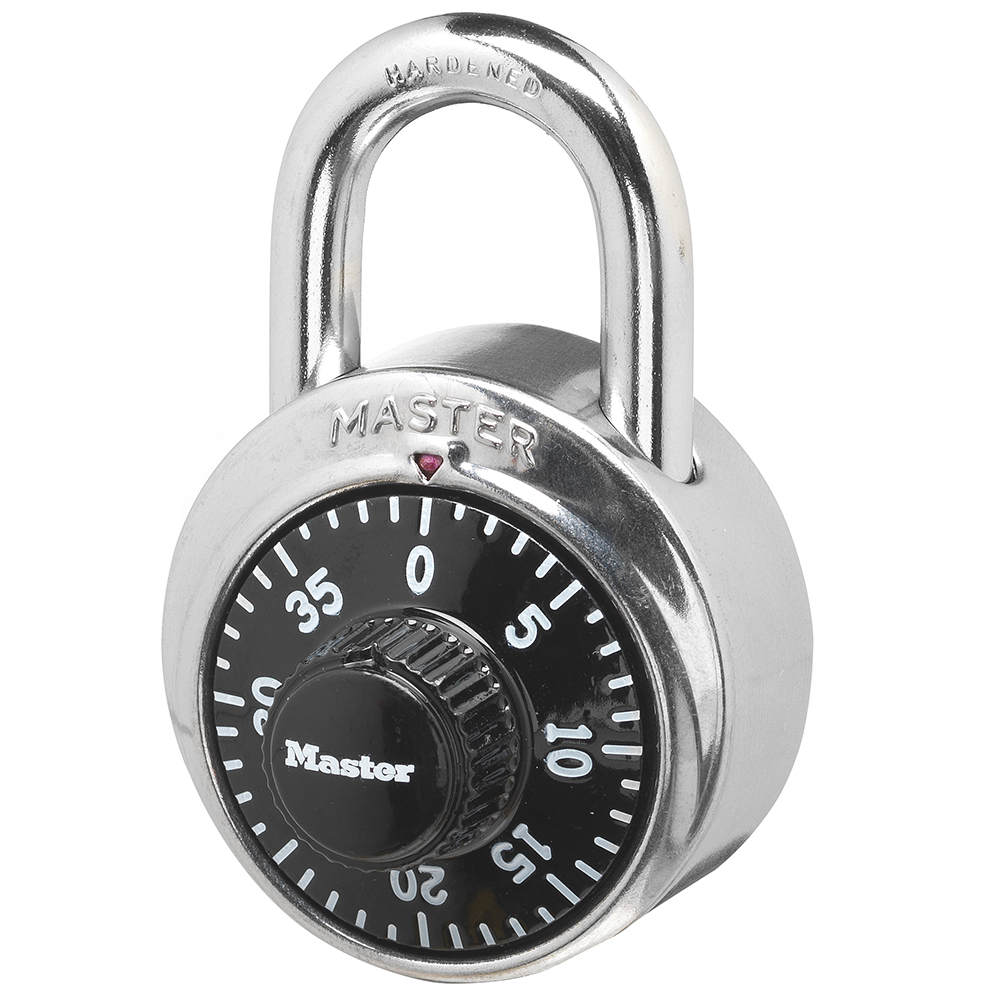
\includegraphics[scale=0.6]{img/C1/1-1/1.png}
    \caption{旋转密码锁}
\end{figure}

如果密码的组合是一个4元组,那么可能的密码组合有$ 40^4 = 2560000 $种。假设尝试一种组合需要花费13秒,一共需要大约9244小时才能尝试完。\\

大部分商业的加密算法是公开的,而军用的加密算法是保密的。\\

\subsection{加密算法}

一种最简单的加密算法就是换位密码/转置密码(Transposition Cipher),它将明文中的字符以某种规则移动位置,形成密文。\\

例如栅栏密码(Rail Fence Cipher),将明文的字符在行与行之间交替,形成密文。\\

比如有一段明文“meet me after the party”,将其分成两行交错排列,得到:\\

m\hspace{0.3cm}e\hspace{0.3cm}m\hspace{0.3cm}a\hspace{0.3cm}t\hspace{0.3cm}r\hspace{0.3cm}h\hspace{0.3cm}p\hspace{0.3cm}r\hspace{0.3cm}y

\hspace{0.4cm}e\hspace{0.4cm}t\hspace{0.4cm}e\hspace{0.3cm}f\hspace{0.4cm}e\hspace{0.3cm}t\hspace{0.3cm}e\hspace{0.3cm}a\hspace{0.3cm}t\\

这种加密方式仅仅只是打乱了顺序,并没有改变明文中的字符和出现频率,因此很容易破解。\\

\subsection{安全性}

加密算法的安全性分为:

\begin{enumerate}
    \item 无条件安全性(unconditionally secure):即使密码分析者拥有无限的计算资源和密文,都没有足够的信息恢复出明文。事实上,只有一次一密乱码本,才是不可破的,对于实际应用的密码算法都是可破的。在实际中,无条件安全的系统是不存在的。
    \item 计算安全性(Computationally secure):当破解所花费的代价远超于被加密信息的生命周期和本身的价值时,破解就失去了意义。
\end{enumerate}

\newpage

\section{凯撒密码}

\subsection{凯撒密码(Caesar Cipher)}

凯撒密码是一种最简单的加密算法,它是由罗马帝国的凯撒(Julius Caesar)发明的。\\

凯撒加密将明文中的字母用另一个字母来替换,替换的规则是将字母向后移动3位。例如,明文中的A将被替换为D,明文中的B将被替换为E,依此类推。

\begin{itemize}
    \item 明文:meet me after the party
    \item 密文:phhw ph diwhu wkh sduwb
\end{itemize}

破解的方法也很容易,只需要将密文的字母向前移动3位即可。\\

改进后的凯撒加密不再采用固定移动3位的策略,而是可以移动任意位数。对于英文字母的加密而言,一个字母可能被替换为另外的25个字母之一。通过暴力枚举每个移位,还是可以破解凯撒加密。\\

\mybox{凯撒密码(加密)}

\begin{lstlisting}[language=Python]
def encrypt(plaintext, shift=3):
    shift %= 26
    ciphertext = ""

    for c in plaintext:
        if not c.isalpha():
            ciphertext += c
            continue
        if c.isupper():
            ciphertext += chr((ord(c) + shift - 65) % 26 + 65)
        else:
            ciphertext += chr((ord(c) + shift - 97) % 26 + 97)

    return ciphertext
\end{lstlisting}

\vspace{0.5cm}

\mybox{凯撒密码(解密)}

\begin{lstlisting}[language=Python]
def decrypt(ciphertext, shift=3):
    plaintext = ""

    for c in ciphertext:
        if not c.isalpha():
            plaintext += c
            continue
        if c.isupper():
            plaintext += chr((ord(c) - shift - 65) % 26 + 65)
        else:
            plaintext += chr((ord(c) - shift - 97) % 26 + 97)

    return plaintext
\end{lstlisting}

\newpage

\section{单表密码}

\subsection{单表密码(Monoalphabetic Cipher)}

单表密码并不像凯撒密码一样仅仅只是将字母后移,而是随机地将一个字母替换为另一个字母。例如字母的替换规则如下:

\begin{table}[H]
    \centering
    \setlength{\tabcolsep}{1mm}{
        \begin{tabular}{|c|c|c|c|c|c|c|c|c|c|c|c|c|c|c|c|c|c|c|c|c|c|c|c|c|c|}
            \hline
            a & b & c & d & e & f & g & h & i & j & k & l & m & n & o & p & q & r & s & t & u & v & w & x & y & z \\
            \hline
            D & K & V & Q & F & I & B & J & W & P & E & S & C & X & H & T & M & Y & A & U & O & L & R & G & Z & N \\
            \hline
        \end{tabular}
    }
\end{table}

\begin{itemize}
    \item 明文:if we wish to replace letters
    \item 密文:WI RF RWAJ UH YFTSDVF SFUUFYA
\end{itemize}

单表密码一共有$ 25! = 1.55 \times 10^{25} $种可能的替换规则,但是它并不安全。由于人类语言的特性,不同的字母的使用频率是不同的。\\

\begin{figure}[H]
    \centering
    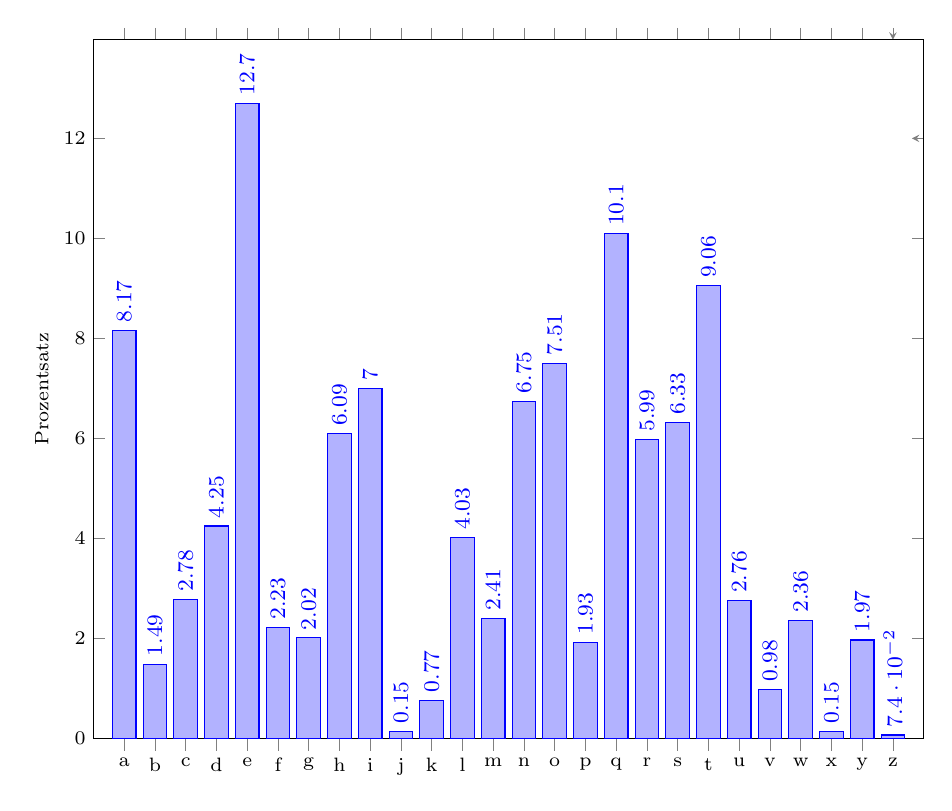
\begin{tikzpicture}
        \scriptsize
        \begin{axis}[width=\linewidth,
                ybar = 1mm,
                bar width = 3mm,
                enlarge x limits=0.04,
                ylabel={Prozentsatz},
                symbolic x coords={a,b,c,d,e,f,g,h,i,j,k,l,m,n,o,p,q,r,s,t,u,v,w,x,y,z},
                xtick=data,
                ymin=0,
                nodes near coords,
                nodes near coords style={rotate=90, anchor=west, font=\footnotesize},
            ]
            \addplot coordinates {
                    (a,8.167)
                    (b,1.492)
                    (c,2.782)
                    (d,4.253)
                    (e,12.702)
                    (f,2.228)
                    (g,2.015)
                    (h,6.094)
                    (i,6.996)
                    (j,0.153)
                    (k,0.772)
                    (l,4.025)
                    (m,2.406)
                    (n,6.749)
                    (o,7.507)
                    (p,1.929)
                    (q,10.095)
                    (r,5.987)
                    (s,6.327)
                    (t,9.056)
                    (u,2.758)
                    (v,0.978)
                    (w,2.360)
                    (x,0.150)
                    (y,1.974)
                    (z,0.074)
                };
        \end{axis}
    \end{tikzpicture}
    \caption{字母使用频率}
\end{figure}

例如有这么一段密文:\\

UZ QSO VUOHXMOPV GPOZPEVSG ZWSZ OPFPESX UDBMETSX

AIZ VUEPHZ HMDZSHZO WSFP APPD TSVP QUZW YMXUZUHSX

EPYEPOPDZSZUFPO MB ZWP FUPZ HMDJ UD TMOHMQ\\

\mybox{字母出现频率}

\begin{lstlisting}[language=Python]
import re

def get_frequency(text):
    frequency = {}
    for c in text:
        if c in frequency:
            frequency[c] += 1
        else:
            frequency[c] = 1
    return frequency


def main():
    with open("ciphertext.txt") as file:
        text = file.readlines()
        text = "".join(text)   
        # remove all non-alphabetic characters
        text = re.sub("[ \n\r]", '', text)

        print(get_frequency(text))


if __name__ == '__main__':
    main()
\end{lstlisting}

这段密文的字母使用频率如下:\\

\{'U': 10, 'Z': 14, 'Q': 3, 'S': 10, 'O': 9, 'V': 5, 'H': 7, 'X': 5, 'M': 8, 'P': 16, 'G': 2, 'E': 6, 'W': 4, 'F': 4, 'D': 6, 'B': 2, 'T': 3, 'A': 2, 'I': 1, 'Y': 2, 'J': 1\}\\

其中P和Z的出现次数最多,分别为16和14次。可以猜测P和Z是对应明文中最常用的字母,因此P和Z非常有可能是e和t。\\

U\textcolor{red}{t} QSO VUOHXMO\textcolor{red}{e}V G\textcolor{red}{e}O\textcolor{red}{t}\textcolor{red}{e}EVSG \textcolor{red}{t}WS\textcolor{red}{t} O\textcolor{red}{e}F\textcolor{red}{e}ESX UDBMETSX

AI\textcolor{red}{t} VUE\textcolor{red}{e}H\textcolor{red}{t} HMD\textcolor{red}{t}SH\textcolor{red}{t}O WSF\textcolor{red}{e} A\textcolor{red}{ee}D TSV\textcolor{red}{e} QU\textcolor{red}{t}W YMXU\textcolor{red}{t}UHSX

E\textcolor{red}{e}YE\textcolor{red}{e}O\textcolor{red}{e}D\textcolor{red}{t}S\textcolor{red}{t}UF\textcolor{red}{e}O MB \textcolor{red}{t}W\textcolor{red}{e} FU\textcolor{red}{et} HMDJ UD TMOHMQ\\

通过英语中单词的组合,可以猜测S对应a、W对应h,因此ZWSZ对应that、ZWP对应the。\\

U\textcolor{red}{t} Q\textcolor{red}{a}O VUOHXMO\textcolor{red}{e}V G\textcolor{red}{e}O\textcolor{red}{t}\textcolor{red}{e}EV\textcolor{red}{a}G \textcolor{red}{that} O\textcolor{red}{e}F\textcolor{red}{e}E\textcolor{red}{a}X UDBMET\textcolor{red}{a}X

AI\textcolor{red}{t} VUE\textcolor{red}{e}H\textcolor{red}{t} HMD\textcolor{red}{ta}H\textcolor{red}{t}O \textcolor{red}{ha}F\textcolor{red}{e} A\textcolor{red}{ee}D T\textcolor{red}{a}V\textcolor{red}{e} QU\textcolor{red}{th} YMXU\textcolor{red}{t}UH\textcolor{red}{a}X

E\textcolor{red}{e}YE\textcolor{red}{e}O\textcolor{red}{e}D\textcolor{red}{ta}\textcolor{red}{t}UF\textcolor{red}{e}O MB \textcolor{red}{the} FU\textcolor{red}{et} HMDJ UD TMOHMQ\\

依次类推,可以破解整个密文:\\

it was disclosed yesterday that several informal

but direct contacts have been made with political

representatives of the viet cong in moscow

\newpage

\section{维吉尼亚密码}

\subsection{维吉尼亚密码(Vigenere Cipher)}

维吉尼亚密码是在凯撒密码的基础上产生的一种加密方法,它将凯撒密码的全部25种位移排序为一张表,与原字母序列共同组成26行26列的密码表。\\

\begin{table}[H]
    \centering
    \setlength{\tabcolsep}{0.5mm}{
        \begin{tabular}{c|c|c|c|c|c|c|c|c|c|c|c|c|c|c|c|c|c|c|c|c|c|c|c|c|c|c|}
                       & \textbf{A} & \textbf{B} & \textbf{C} & \textbf{D} & \textbf{E} & \textbf{F} & \textbf{G} & \textbf{H} & \textbf{I} & \textbf{J} & \textbf{K} & \textbf{L} & \textbf{M} & \textbf{N} & \textbf{O} & \textbf{P} & \textbf{Q} & \textbf{R} & \textbf{S} & \textbf{T} & \textbf{U} & \textbf{V} & \textbf{W} & \textbf{X} & \textbf{Y} & \textbf{Z} \\
            \hline
            \textbf{A} & A          & B          & C          & D          & E          & F          & G          & H          & I          & J          & K          & L          & M          & N          & O          & P          & Q          & R          & S          & T          & U          & V          & W          & X          & Y          & Z          \\[-1ex]
            \hline
            \textbf{B} & B          & C          & D          & E          & F          & G          & H          & I          & J          & K          & L          & M          & N          & O          & P          & Q          & R          & S          & T          & U          & V          & W          & X          & Y          & Z          & A          \\[-1ex]
            \hline
            \textbf{C} & C          & D          & E          & F          & G          & H          & I          & J          & K          & L          & M          & N          & O          & P          & Q          & R          & S          & T          & U          & V          & W          & X          & Y          & Z          & A          & B          \\[-1ex]
            \hline
            \textbf{D} & D          & E          & F          & G          & H          & I          & J          & K          & L          & M          & N          & O          & P          & Q          & R          & S          & T          & U          & V          & W          & X          & Y          & Z          & A          & B          & C          \\[-1ex]
            \hline
            \textbf{E} & E          & F          & G          & H          & I          & J          & K          & L          & M          & N          & O          & P          & Q          & R          & S          & T          & U          & V          & W          & X          & Y          & Z          & A          & B          & C          & D          \\[-1ex]
            \hline
            \textbf{F} & F          & G          & H          & I          & J          & K          & L          & M          & N          & O          & P          & Q          & R          & S          & T          & U          & V          & W          & X          & Y          & Z          & A          & B          & C          & D          & E          \\[-1ex]
            \hline
            \textbf{G} & G          & H          & I          & J          & K          & L          & M          & N          & O          & P          & Q          & R          & S          & T          & U          & V          & W          & X          & Y          & Z          & A          & B          & C          & D          & E          & F          \\[-1ex]
            \hline
            \textbf{H} & H          & I          & J          & K          & L          & M          & N          & O          & P          & Q          & R          & S          & T          & U          & V          & W          & X          & Y          & Z          & A          & B          & C          & D          & E          & F          & G          \\[-1ex]
            \hline
            \textbf{I} & I          & J          & K          & L          & M          & N          & O          & P          & Q          & R          & S          & T          & U          & V          & W          & X          & Y          & Z          & A          & B          & C          & D          & E          & F          & G          & H          \\[-1ex]
            \hline
            \textbf{J} & J          & K          & L          & M          & N          & O          & P          & Q          & R          & S          & T          & U          & V          & W          & X          & Y          & Z          & A          & B          & C          & D          & E          & F          & G          & H          & I          \\[-1ex]
            \hline
            \textbf{K} & K          & L          & M          & N          & O          & P          & Q          & R          & S          & T          & U          & V          & W          & X          & Y          & Z          & A          & B          & C          & D          & E          & F          & G          & H          & I          & J          \\[-1ex]
            \hline
            \textbf{L} & L          & M          & N          & O          & P          & Q          & R          & S          & T          & U          & V          & W          & X          & Y          & Z          & A          & B          & C          & D          & E          & F          & G          & H          & I          & J          & K          \\[-1ex]
            \hline
            \textbf{M} & M          & N          & O          & P          & Q          & R          & S          & T          & U          & V          & W          & X          & Y          & Z          & A          & B          & C          & D          & E          & F          & G          & H          & I          & J          & K          & L          \\[-1ex]
            \hline
            \textbf{N} & N          & O          & P          & Q          & R          & S          & T          & U          & V          & W          & X          & Y          & Z          & A          & B          & C          & D          & E          & F          & G          & H          & I          & J          & K          & L          & M          \\[-1ex]
            \hline
            \textbf{O} & O          & P          & Q          & R          & S          & T          & U          & V          & W          & X          & Y          & Z          & A          & B          & C          & D          & E          & F          & G          & H          & I          & J          & K          & L          & M          & N          \\[-1ex]
            \hline
            \textbf{P} & P          & Q          & R          & S          & T          & U          & V          & W          & X          & Y          & Z          & A          & B          & C          & D          & E          & F          & G          & H          & I          & J          & K          & L          & M          & N          & O          \\[-1ex]
            \hline
            \textbf{Q} & Q          & R          & S          & T          & U          & V          & W          & X          & Y          & Z          & A          & B          & C          & D          & E          & F          & G          & H          & I          & J          & K          & L          & M          & N          & O          & P          \\[-1ex]
            \hline
            \textbf{R} & R          & S          & T          & U          & V          & W          & X          & Y          & Z          & A          & B          & C          & D          & E          & F          & G          & H          & I          & J          & K          & L          & M          & N          & O          & P          & Q          \\[-1ex]
            \hline
            \textbf{S} & S          & T          & U          & V          & W          & X          & Y          & Z          & A          & B          & C          & D          & E          & F          & G          & H          & I          & J          & K          & L          & M          & N          & O          & P          & Q          & R          \\[-1ex]
            \hline
            \textbf{T} & T          & U          & V          & W          & X          & Y          & Z          & A          & B          & C          & D          & E          & F          & G          & H          & I          & J          & K          & L          & M          & N          & O          & P          & Q          & R          & S          \\[-1ex]
            \hline
            \textbf{U} & U          & V          & W          & X          & Y          & Z          & A          & B          & C          & D          & E          & F          & G          & H          & I          & J          & K          & L          & M          & N          & O          & P          & Q          & R          & S          & T          \\[-1ex]
            \hline
            \textbf{V} & V          & W          & X          & Y          & Z          & A          & B          & C          & D          & E          & F          & G          & H          & I          & J          & K          & L          & M          & N          & O          & P          & Q          & R          & S          & T          & U          \\[-1ex]
            \hline
            \textbf{W} & W          & X          & Y          & Z          & A          & B          & C          & D          & E          & F          & G          & H          & I          & J          & K          & L          & M          & N          & O          & P          & Q          & R          & S          & T          & U          & V          \\[-1ex]
            \hline
            \textbf{X} & X          & Y          & Z          & A          & B          & C          & D          & E          & F          & G          & H          & I          & J          & K          & L          & M          & N          & O          & P          & Q          & R          & S          & T          & U          & V          & W          \\[-1ex]
            \hline
            \textbf{Y} & Y          & Z          & A          & B          & C          & D          & E          & F          & G          & H          & I          & J          & K          & L          & M          & N          & O          & P          & Q          & R          & S          & T          & U          & V          & W          & X          \\[-1ex]
            \hline
            \textbf{Z} & Z          & A          & B          & C          & D          & E          & F          & G          & H          & I          & J          & K          & L          & M          & N          & O          & P          & Q          & R          & S          & T          & U          & V          & W          & X          & Y          \\[-1ex]
            \hline
        \end{tabular}
    }
    \caption{维吉尼亚密码表}
\end{table}

除了密码表,还必须有一个密钥(key)。密钥由字母组成,最少一个字母,最多可与明文字母数相等。如果密钥只有1个字母,相当于凯撒密码。\\

\subsection{加密}

例如:

\begin{itemize}
    \item 明文:I Love You
    \item 密钥:OK
\end{itemize}

首先,如果密钥长度小于明文长度(非字母忽略),就重复拼接密钥,使其与明文长度相等。

\begin{itemize}
    \item 明文:I Love You
    \item 密钥:OKOKOKOK
\end{itemize}

接着根据密码表进行加密。明文第一个字母是I,密钥的第一个字母是O,因此在查找密码表的I行O列,得到加密后的字母W。同理,第二个字母为位于L行K列的字母V。\\

依次类推,得到密文:W VCFS ICE。\\

\subsection{解密}

例如:

\begin{itemize}
    \item 密文:PWZRNZBZEANQKBUHNLNB
    \item 密钥:WIND
\end{itemize}

首先把密钥重复拼接,直到和密文长度相同。

\begin{itemize}
    \item 密文:PWZRNZBZEANQKBUHNLNB
    \item 密钥:WINDWINDWINDWINDWIND
\end{itemize}

根据密文的第一个字母P,在密码表中找到P行,在P行找出值为W的列,沿着该列向上找到该列为T,因此P解密后可以得到T。\\

根据相同的方法,可以得到明文:TOMORROWISANOTHERDAY。\\

\mybox{维吉尼亚密码}

\begin{lstlisting}[language=Python]
import re

def generate_key(plaintext, key):
    n = len(plaintext) - len(key)
    for i in range(n): 
        key += key[i % len(key)]
    return key


def encrypt(plaintext, key):
    # remove all non-alphabetic characters
    plaintext = re.sub("[ \n\r]", '', plaintext).upper()
    key = generate_key(plaintext, key)

    ciphertext = ""
    for i in range(len(plaintext)):
        ciphertext += chr((ord(plaintext[i]) + ord(key[i])) % 26 + 65)
    return ciphertext


def decrypt(ciphertext, key):
    # remove all non-alphabetic characters
    ciphertext = re.sub("[ \n\r]", '', ciphertext).upper()
    key = generate_key(ciphertext, key)

    plaintext = ""
    for i in range(len(ciphertext)):
        plaintext += chr((ord(ciphertext[i]) - ord(key[i])) % 26 + 65)
    return plaintext
\end{lstlisting}

\newpage

\section{一次性密码本}

\subsection{一次性密码本(One-Time Pad)}

一次性密码本算法所用的密钥是一次性的,因此不会出现因为密钥泄露导致之前的加密内容被破解的情况。即使密钥被泄露了,也只会影响一次通信过程。\\

计算机在传输数据时,会将文字转换为对应的二进制编码。通过随机生成一个与明文的二进制编码长度相同的密钥,一次性密码本将明文和密钥进行异或(XOR)运算,得到密文。\\

由于XOR运算的特性,即比特位相同为0,不同为1:

\begin{itemize}
    \item 0 XOR 0 = 0
    \item 0 XOR 1 = 1
    \item 1 XOR 0 = 1
    \item 1 XOR 1 = 0
\end{itemize}

同时另一个XOR的特性就是可逆性,即A XOR B = C,则C XOR B = A。那么通过将密文和密钥再次异或操作就可以得到原文。\\

\subsection{优势}

虽然一次性密码本非常简单,但是一次性密码本是无法破译的,这个破译并不是指现有的计算能力不够,而是指即使拥有无穷大的计算能力也无法破译。\\

假如你拿到了一段128 bits的密文,通过遍历等长的密钥进行暴力破解,将会生成$ 2^{128} $个原文,即原文的所有排列组合。\\

在这些排列组合中,可能会出现一些有意义的文字,但是你并不能确定这些文字是否就是原文,因为在所有的排列组合中会产生大量有意义的问题。\\

因此破解一次性密码本算法是无意义的,就像是知道了原文的长度,然后自己构造了一个这个长度的原文。\\

\subsection{缺陷}

既然一次性密码本这么好,那么为什么我们在实际中很少用到呢?

\begin{itemize}
    \item 密钥太长:密钥的长度与原文相同,如果原文很大,那么对应的密钥也很大。

    \item 密钥无法重用:每个密钥只用一次,既是优点也是缺点。这意味着每次都要不停地更换密钥,增加了复杂性。

    \item 密钥的配送:目标端如果想解密就必须拿到密钥,如果能够机密地传输密钥给目标端,那为什么不直接将原文机密地传送给目标端呢?

    \item 密钥的保存:每一个明文都需要保存一个同样长度的密钥。
\end{itemize}

\newpage

\section{Playfair密码}

\subsection{Playfair密码(Playfair Cipher)}

Playfair密码是一种使用一个关键词方格来加密字符对的加密法,在1854年由Charles Wheatstone发明。曾在一战时期被英军所使用,二战时期澳大利亚所使用。\\

首先选取一个英文单词作为密钥,将这个单词(去除重复字母)填入一个$ 5 \times 5 $的矩阵中,剩余的位置按照字母表顺序填入方格中,其中$ I $和$ J $视作同一个字母。\\

例如选取单词PLAYFAIR作为密钥,生成的密钥矩阵如下:

\[
    \begin{bmatrix}
        P & L & A & Y & F \\
        I & R & B & C & D \\
        E & G & H & K & M \\
        N & O & Q & S & T \\
        U & V & W & X & Z
    \end{bmatrix}
\]

\vspace{0.5cm}

假设需要加密的明文为HELLO THERE,将明文中的字符两两配对。当一对中出现两个相同字母时,用x分隔。当最后一对只剩一个字母时,也是用x配对。

\begin{itemize}
    \item 明文:HELLO THERE
    \item 配对:HE LX LO TH ER EX
\end{itemize}

对于每一对字母,如果它们在密钥矩阵中位于同一行,将它们替换为各自右边的字母,如HE加密为KG。如果它们位于同一列,将它们替换为各自下面的字母,如LO加密为RV。其它情况,将它们的列下标互换,如LX加密为YV。

\begin{itemize}
    \item 密文:KG YV RV QM GI KU
\end{itemize}

\vspace{0.5cm}

\subsection{解密}

假设目前截获了一份使用Playfair加密的密文和对应的原文,以及一个不完整的密钥矩阵,现在需要对另一份密文进行解密。

\begin{itemize}
    \item 明文:THE QUICK BROWN FOX JUMPS OVER THE LAZY DOG
    \item 密文:RMAPLHBMUAWRVDPWHLISNPXGEGIRBEVZHNEV
    \item 待解密密文:RMTGNTEATG
    \item 不完整的密钥矩阵:
\end{itemize}

\[
    \begin{bmatrix}
          &   &   & A & T \\
          & U &   & B & C \\
          &   & I &   &   \\
        N &   & P &   & S \\
          & W &   &   & Z
    \end{bmatrix}
\]

\vspace{0.5cm}

解密的方法就是根据已有的一组明文和密文,推算出完整的密钥矩阵。再根据密钥矩阵,反向利用Playfair的加密方法进行解密。\\

首先将已有的明文和密文进行两两匹配:

\begin{itemize}
    \item 明文:TH EQ UI CK BR OW NF OX JU MP SO VE RT HE LA ZY DO GX
    \item 密文:RM AP LH BM UA WR VD PW HL IS NP XG EG IR BE VZ HN EV
\end{itemize}

可以发现在这些配对中,有些配对在明文和密文中出现了相同的字母:

\begin{itemize}
    \item 明文:TH EQ UI CK BR \textcolor{red}{OW} NF OX JU MP SO VE RT HE LA \textcolor{blue}{ZY} DO GX
    \item 密文:RM AP LH BM UA \textcolor{red}{WR} VD PW HL IS NP XG EG IR BE \textcolor{blue}{VZ} HN EV
\end{itemize}

这种情况只有可能发现在被加密的两个字母出现在相邻的位置上,这样被加密时,使用它们各自右边或下面的字母,就会出现重复。\\

根据这个信息,可以推算出$ V $、$ Y $、$ R $、$ O $的位置。

\[
    \begin{bmatrix}
                            & \textcolor{red}{R} &   & A                   & T \\
                            & U                  &   & B                   & C \\
                            &                    & I &                     &   \\
        N                   & \textcolor{red}{O} & P &                     & S \\
        \textcolor{blue}{V} & W                  &   & \textcolor{blue}{Y} & Z
    \end{bmatrix}
\]

\vspace{0.5cm}

由于秘钥矩阵后,后面的字母都是按照字母表的顺序排列的,所以推算出一部分缺失的字母。

\[
    \begin{bmatrix}
          & R &                    & A                  & T \\
          & U &                    & B                  & C \\
          &   & I                  &                    &   \\
        N & O & P                  & \textcolor{red}{Q} & S \\
        V & W & \textcolor{red}{X} & Y                  & Z
    \end{bmatrix}
\]

\vspace{0.5cm}

再次根据已有的明文和密文,可以推算出其它字母的位置。

\begin{itemize}
    \item 明文:\textcolor{red}{TH} \textcolor{blue}{EQ} \textcolor{green}{UI} \textcolor{cyan}{CK} BR OW NF OX JU MP SO \textcolor{brown}{VE} RT HE LA ZY \textcolor{purple}{DO} GX
    \item 密文:\textcolor{red}{RM} \textcolor{blue}{AP} \textcolor{green}{LH} \textcolor{cyan}{BM} UA WR VD PW HL IS NP \textcolor{brown}{XG} EG IR BE VZ \textcolor{purple}{HN} EV
\end{itemize}

\[
    \begin{bmatrix}
        \textcolor{brown}{G}  & R                  & \textcolor{blue}{E}  & A                   & T                  \\
        \textcolor{pink}{F}   & U                  & \textcolor{green}{L} & B                   & C                  \\
        \textcolor{purple}{D} & \textcolor{red}{H} & I                    & \textcolor{cyan}{K} & \textcolor{red}{M} \\
        N                     & O                  & P                    & Q                   & S                  \\
        V                     & W                  & X                    & Y                   & Z
    \end{bmatrix}
\]

\vspace{0.5cm}

在破解出完整的密钥矩阵后,就可以利用Playfair的解密方法对密文RMTGNTEATG解密了。

\begin{itemize}
    \item 密文:RM TG NT EA TG
    \item 明文:TH AT SG RE AT
\end{itemize}

\newpage
\chapter{数论}


\chapter{现代密码学}

\section{RSA}

\subsection{RSA}

RSA是一种非对称加密(asymmetric cryptography)算法,在1977年由Ron Rivest、Adi ShamirLeonard Adleman一起提出,RSA就是他们三人姓氏的首字母。\\

所谓非对称加密,是指在网络通信中双方各有一对密钥,其中公钥(public key)被公开给外界,用于加密;私钥(private key)只有自己知道,用于解密。\\

例如Alice的一组密钥为$ (P_A, S_A) $,Bob的一组密钥为$ (P_B, S_B) $。对一段消息$ M $加密和解密的操作是互逆的:

\vspace{-1cm}

\begin{align*}
    M & = S_A(P_A(M)) \\
    M & = P_A(S_A(M))
\end{align*}

如果Bob想要给Alice发送消息,Bob首先使用Alice的公钥$ P_A $对消息$ M $进行加密得到密文$ C $:

\vspace{-1cm}

\begin{align*}
    C = P_A(M)
\end{align*}

Bob将密文$ C $发送给Alice,Alice使用自己的私钥$ S_A $对密文$ C $进行解密得到原文$ M $:

\vspace{-1cm}

\begin{align*}
    S_A(C) = S_A(P_A(M)) = M
\end{align*}

\vspace{0.5cm}

\subsection{公钥/私钥生成}

RSA的安全性依赖于大整数的质因数分解,也就是对于两个大素数$ p $和$ q $而言,计算它们的乘积$ pq $很容易,但是从积$ pq $分解出$ p $和$ q $是个公认的数学难题。\\

RSA公钥和私钥生成的过程如下:

\begin{enumerate}
    \item 随机选择两个大素数(超过100位),为了简化说明,这里采用较小的素数$ p = 41 $、$ q = 59 $

    \item 计算$ p $和$ q $的乘积$ n = pq = 2419 $

    \item 计算$ p - 1 $与$ q - 1 $的乘积$ \phi(n) = (p-1)(q-1) = 40 * 58 = 2320 $

    \item 选择一个小奇数$ e $,使得$ gcd(e, \phi(n)) = 1$,例如$ e = 3 $

    \item 计算$ d $,使得$ d * e \equiv 1\ (\text{mod}\ \phi(n)) $。当$ d = 1547 $时,$ 1547 * 3\ \text{mod}\ 2320 = 1 $

    \item 公钥$ P = (e, n) = (3, 2419) $

    \item 私钥$ S = (d, n) = (1547, 2419) $

    \item 对消息$ M $加密的过程为$ P(M) = M^e\ (\text{mod}\ n) = M^3\ (\text{mod}\ 2419) $

    \item 对消息$ M $解密的过程为$ S(M) = M^d\ (\text{mod}\ n) = M^{1547}\ (\text{mod}\ 2419) $
\end{enumerate}

\vspace{0.5cm}

\subsection{加密}

假设Alice的公钥为$ (9, 2419) $,想要将消息“PACE”发送给Bob。\\

首先将消息中的英文字母转换为对应的编码:

\begin{itemize}
    \item PA = 1500
    \item CE = 0204
\end{itemize}

\begin{table}[H]
    \centering
    \setlength{\tabcolsep}{5mm}{
        \begin{tabular}{|c|c|c|c|}
            \hline
            \textbf{Letter} & \textbf{Code} & \textbf{Letter} & \textbf{Code} \\
            \hline
            A               & 00            & B               & 01            \\
            \hline
            C               & 02            & D               & 03            \\
            \hline
            E               & 04            & F               & 05            \\
            \hline
            G               & 06            & H               & 07            \\
            \hline
            I               & 08            & J               & 09            \\
            \hline
            K               & 10            & L               & 11            \\
            \hline
            M               & 12            & N               & 13            \\
            \hline
            O               & 14            & P               & 15            \\
            \hline
            Q               & 16            & R               & 17            \\
            \hline
            S               & 18            & T               & 19            \\
            \hline
            U               & 20            & V               & 21            \\
            \hline
            W               & 22            & X               & 23            \\
            \hline
            Y               & 24            & Z               & 25            \\
            \hline
        \end{tabular}
    }
\end{table}

分别对PA和CE进行加密:

\begin{itemize}
    \item $ P(1500) = 1500^9\ (\text{mod}\ 2419) = 1655 $
    \item $ P(0204) = 204^9\ (\text{mod}\ 2419) = 1639 $
\end{itemize}

最终形成的密文为1655 1639。

\newpage

\section{DES}

\subsection{DES(Data Encryption Standard)}

DES是一种分组密码,它将数据分成多个64位的块,每个块独立加密。因此,DES将64位的明文作为输入,输出64位的密文。\\

DES首先需要对原始数据进行一次初始置换(IP, Initial Permutation),接着进行16轮迭代运算,对数据重新排列和置换,最后再对数据进行一次最终置换(FP, Final Permutation),得到最终的密文。\\

\begin{figure}[H]
    \centering
    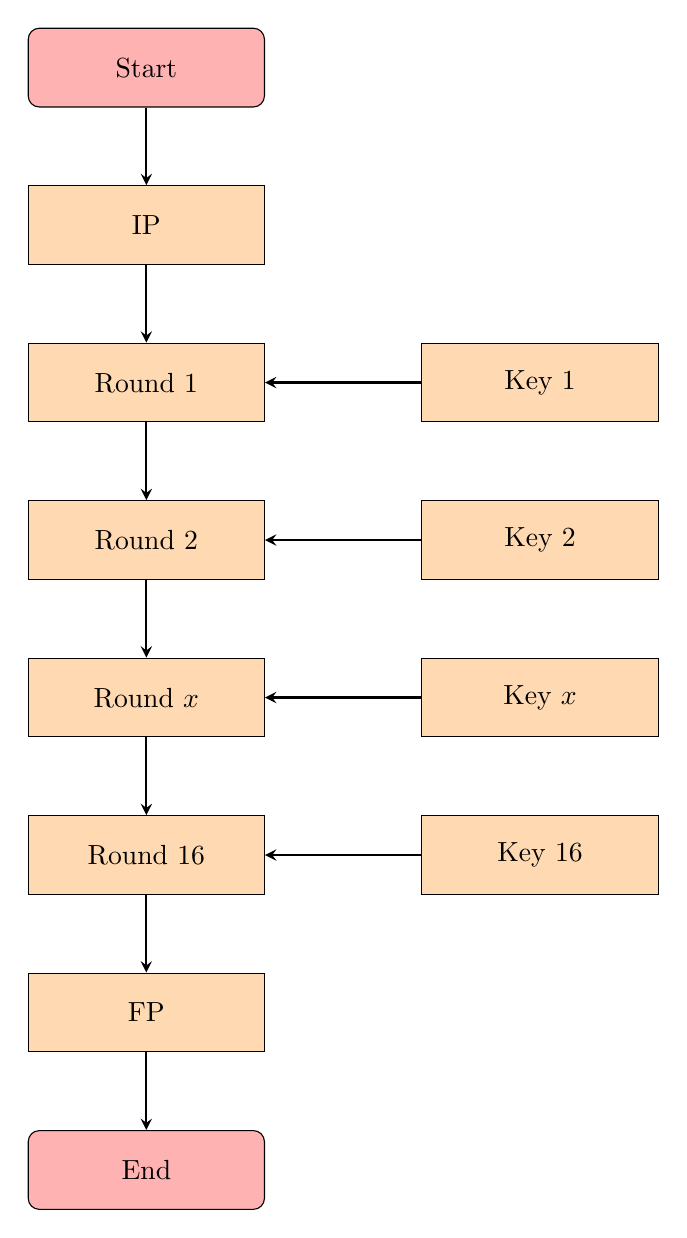
\begin{tikzpicture}[node distance=2cm]
        \node (start) [startend] {Start};
        \node (IP) [process, below of=start] {IP};
        \node (round1) [process, below of=IP] {Round 1};
        \node (key1) [process, right of=round1, xshift=3cm] {Key 1};
        \node (round2) [process, below of=round1] {Round 2};
        \node (key2) [process, right of=round2, xshift=3cm] {Key 2};
        \node (roundx) [process, below of=round2] {Round $ x $};
        \node (keyx) [process, right of=roundx, xshift=3cm] {Key $ x $};
        \node (round16) [process, below of=roundx] {Round 16};
        \node (key16) [process, right of=round16, xshift=3cm] {Key 16};
        \node (FP) [process, below of=round16] {FP};
        \node (end) [startend, below of=FP] {End};

        \draw [arrow] (start) -- (IP);
        \draw [arrow] (IP) -- (round1);
        \draw [arrow] (key1) -- (round1);
        \draw [arrow] (key2) -- (round2);
        \draw [arrow] (round1) -- (round2);
        \draw [arrow] (round2) -- (roundx);
        \draw [arrow] (keyx) -- (roundx);
        \draw [arrow] (roundx) -- (round16);
        \draw [arrow] (key16) -- (round16);
        \draw [arrow] (round16) -- (FP);
        \draw [arrow] (FP) -- (end);
    \end{tikzpicture}
    \caption{DES}
\end{figure}

\vspace{0.5cm}

\subsection{密钥生成}

由于在DES的16轮迭代加密的过程中,每一轮都需要使用一个不同的密钥。因此,在DES开始加密之前,需要先根据原始的密钥,生成16个不同的密钥。\\

原始的密钥的长度为64位,其中第8、16、24、32、40、48、56、64位为奇偶校验位。因此,忽略这8位奇偶校验位,然后对剩余的56位进行重新排列,排列的顺序参照PC-1。\\

\begin{table}[H]
    \centering
    \setlength{\tabcolsep}{5mm}{
        \begin{tabular}{|c|c|c|c|c|c|c|}
            \hline
            57 & 49 & 41 & 33 & 25 & 17 & 9  \\
            \hline
            1  & 58 & 50 & 42 & 34 & 26 & 18 \\
            \hline
            10 & 2  & 59 & 51 & 43 & 35 & 27 \\
            \hline
            19 & 11 & 3  & 60 & 52 & 44 & 36 \\
            \hline
            63 & 55 & 47 & 39 & 31 & 23 & 15 \\
            \hline
            7  & 62 & 54 & 46 & 38 & 30 & 22 \\
            \hline
            14 & 6  & 61 & 53 & 45 & 37 & 29 \\
            \hline
            21 & 13 & 5  & 28 & 20 & 12 & 4  \\
            \hline
        \end{tabular}
    }
    \caption{PC-1}
\end{table}

其中PC-1的每个数字代表依次排列的位置,例如57代表将原始密钥第57位放到第1位,40代表将原始密钥第40位放到第2位,依次类推。由于PC-1表中只包含56个位置,在进行重新选择排列的过程中,即可忽略掉8位奇偶校验位。\\

例如原始密钥为:

\begin{verbatim}
    00010011 00110100
    01010111 01111001
    10011011 10111100
    11011111 11110001
\end{verbatim}

重新选择排列后得到一个56位的密钥:

\begin{verbatim}
    1111000 0110011
    0010101 0101111
    0101010 1011001
    1001111 0001111
\end{verbatim}

接着将56位的密钥分为两部分,分别为左28位和右28位,分别对它们进行16次循环左移,循环左移的次数参照移位表。\\

\begin{table}[H]
    \centering
    \setlength{\tabcolsep}{2mm}{
        \begin{tabular}{|c|c|c|c|c|c|c|c|c|c|c|c|c|c|c|c|c|}
            \hline
            \textbf{第$ i $轮}    & 1 & 2 & 3 & 4 & 5 & 6 & 7 & 8 & 9 & 10 & 11 & 12 & 13 & 14 & 15 & 16 \\
            \hline
            \textbf{循环左移位数} & 1 & 1 & 2 & 2 & 2 & 2 & 2 & 2 & 1 & 2  & 2  & 2  & 2  & 2  & 2  & 1  \\
            \hline
        \end{tabular}
    }
    \caption{移位表}
\end{table}

在每一轮循环左移后,将左右两部分重新,拼接成一个56位的密钥,然后对这个56位的密钥进行重新选择排列,最终生成每一轮的48位密钥,排列的顺序参照PC-2。\\

\begin{table}[H]
    \centering
    \setlength{\tabcolsep}{5mm}{
        \begin{tabular}{|c|c|c|c|c|c|}
            \hline
            14 & 17 & 11 & 24 & 1  & 5  \\
            \hline
            3  & 28 & 15 & 6  & 21 & 10 \\
            \hline
            23 & 19 & 12 & 4  & 26 & 8  \\
            \hline
            16 & 7  & 27 & 20 & 13 & 2  \\
            \hline
            41 & 52 & 31 & 37 & 47 & 55 \\
            \hline
            30 & 40 & 51 & 45 & 33 & 48 \\
            \hline
            44 & 49 & 39 & 56 & 34 & 53 \\
            \hline
            46 & 42 & 50 & 36 & 29 & 32 \\
            \hline
        \end{tabular}
    }
    \caption{PC-2}
\end{table}

\vspace{0.5cm}

\subsection{IP置换}

在生成16个密钥后,就可以对明文进行加密了。第一步需要先对明文进行IP置换,IP置换的顺序参照IP表。\\

\begin{table}[H]
    \centering
    \setlength{\tabcolsep}{5mm}{
        \begin{tabular}{|c|c|c|c|c|c|c|c|}
            \hline
            58 & 50 & 42 & 34 & 26 & 18 & 10 & 2 \\
            \hline
            60 & 52 & 44 & 36 & 28 & 20 & 12 & 4 \\
            \hline
            62 & 54 & 46 & 38 & 30 & 22 & 14 & 6 \\
            \hline
            64 & 56 & 48 & 40 & 32 & 24 & 16 & 8 \\
            \hline
            57 & 49 & 41 & 33 & 25 & 17 & 9  & 1 \\
            \hline
            59 & 51 & 43 & 35 & 27 & 19 & 11 & 3 \\
            \hline
            61 & 53 & 45 & 37 & 29 & 21 & 13 & 5 \\
            \hline
            63 & 55 & 47 & 39 & 31 & 23 & 15 & 7 \\
            \hline
        \end{tabular}
    }
    \caption{IP}
\end{table}

\vspace{0.5cm}

\subsection{16轮迭代}

将置换后的64位明文分为左32位和右32位,然后进行16轮迭代加密,每一轮的处理过程如下:\\

\begin{figure}[H]
    \centering
    \begin{tikzpicture}
        \draw (0,10) rectangle (3,10.75) node[xshift=-1.5cm, yshift=-0.5cm] {$ L_0 $};
        \draw (7,10) rectangle (10,10.75) node[xshift=-1.5cm, yshift=-0.5cm] {$ R_0 $};

        \node[draw, trapezium] (E) at (8.5,8.5) {E扩展};
        \node [XORgate] at (8.5,7) (XOR1) {\large +};
        \node[draw, trapezium, rotate=180] (S) at (8.5,5.5) {\textcolor{white}{S盒}};
        \node at (8.5,5.5) {S盒};
        \node[draw, rectangle] (P) at (8.5,4) {P盒};
        \node [XORgate] at (8.5,2.25) (XOR2) {\large +};

        \draw (0,0) rectangle (3,0.75) node[xshift=-1.5cm, yshift=-0.5cm] {$ L_1 $};
        \draw (7,0) rectangle (10,0.75) node[xshift=-1.5cm, yshift=-0.5cm] {$ R_1 $};

        \draw (11,7) node[right] {$ key_i $} -- (XOR1);
        \node at (10,6.7) {48};

        \draw (1.5,10) node[right, yshift=-0.5cm] {32} -- (1.5,4) -- (XOR2);
        \draw (8.5,10) node[right, yshift=-0.5cm] {32} -- (E);
        \draw (8.5,9.5) -- (6,9) -- (1.5,0.75) node[above, yshift=0.3cm] {32};
        \draw (E) -- (XOR1) node[left, xshift=-0.2cm, yshift=0.7cm] {48};
        \draw (XOR1) -- (S) node[left, xshift=-0.2cm, yshift=0.7cm] {48};
        \draw (S) -- (P) node[left, xshift=-0.2cm, yshift=0.7cm] {32};
        \draw (P) -- (XOR2) node[left, xshift=-0.2cm, yshift=0.8cm] {32};
        \draw (XOR2) -- (8.5,0.75) node[left, xshift=-0.2cm, yshift=0.5cm] {32};
    \end{tikzpicture}
    \caption{16轮迭代}
\end{figure}

\vspace{0.5cm}

\subsection{E扩展(Expansion Permutation)}

E扩展将32位的右半部分扩展为48位,扩展的顺序参照E表。\\

\begin{table}[H]
    \centering
    \setlength{\tabcolsep}{5mm}{
        \begin{tabular}{|c|c|c|c|c|c|c|c|}
            \hline
            32 & 1  & 2  & 3  & 4  & 5  & 4  & 5  \\
            \hline
            6  & 7  & 8  & 9  & 8  & 9  & 10 & 11 \\
            \hline
            12 & 13 & 12 & 13 & 14 & 15 & 16 & 17 \\
            \hline
            16 & 17 & 18 & 19 & 20 & 21 & 20 & 21 \\
            \hline
            22 & 23 & 24 & 25 & 24 & 25 & 26 & 27 \\
            \hline
            28 & 29 & 28 & 29 & 30 & 31 & 32 & 1  \\
            \hline
        \end{tabular}
    }
    \caption{E}
\end{table}

E扩展的规则其实是将原来的32位以4位一组划分,然后将每一组的最后一位复制到后一组的前面,将每一组的第一位复制到前一组的后面,(其中第一组的前一组为最后一组,最后一组的下一组为第一组)。\\

这样就可以将4位一组扩展为6位一组,最后按顺序合并,即可得到48位的结果。\\

最后将扩展完的48位与之前生成的该轮密钥进行异或运算,得到48位的结果。\\

\subsection{S盒(S-Box Substitution)}

S盒用于将48位的数据压缩为32位。首先将48位的数据分为8组,每组6位,每一组都会根据对应的S盒(共8个,$ S_1 \sim S_8 $)进行压缩。因此,每个S盒都需要将6位输入压缩为4位输出。\\

每个S盒都由4行16列组成:\\

\begin{table}[H]
    \centering
    \setlength{\tabcolsep}{2mm}{
        \begin{tabular}{|c|c|c|c|c|c|c|c|c|c|c|c|c|c|c|c|c|}
            \hline
                       & \textbf{0} & \textbf{1} & \textbf{2} & \textbf{3} & \textbf{4} & \textbf{5} & \textbf{6} & \textbf{7} & \textbf{8} & \textbf{9} & \textbf{10} & \textbf{11} & \textbf{12} & \textbf{13} & \textbf{14} & \textbf{15} \\
            \hline
            \textbf{0} & 14         & 4          & 13         & 1          & 2          & 15         & 11         & 8          & 3          & 10         & 6           & 12          & 5           & 9           & 0           & 7           \\
            \hline
            \textbf{1} & 0          & 15         & 7          & 4          & 14         & 2          & 13         & 1          & 10         & 6          & 12          & 11          & 9           & 5           & 3           & 8           \\
            \hline
            \textbf{2} & 4          & 1          & 14         & 8          & 13         & 6          & 2          & 11         & 15         & 12         & 9           & 7           & 3           & 10          & 5           & 0           \\
            \hline
            \textbf{3} & 15         & 12         & 8          & 2          & 4          & 9          & 1          & 7          & 5          & 11         & 3           & 14          & 10          & 0           & 6           & 13          \\
            \hline
        \end{tabular}
    }
    \caption{$ S_1 $}
\end{table}

\begin{table}[H]
    \centering
    \setlength{\tabcolsep}{2mm}{
        \begin{tabular}{|c|c|c|c|c|c|c|c|c|c|c|c|c|c|c|c|c|}
            \hline
                       & \textbf{0} & \textbf{1} & \textbf{2} & \textbf{3} & \textbf{4} & \textbf{5} & \textbf{6} & \textbf{7} & \textbf{8} & \textbf{9} & \textbf{10} & \textbf{11} & \textbf{12} & \textbf{13} & \textbf{14} & \textbf{15} \\
            \hline
            \textbf{0} & 15         & 1          & 8          & 14         & 6          & 11         & 3          & 4          & 9          & 7          & 2           & 13          & 12          & 0           & 5           & 10          \\
            \hline
            \textbf{1} & 3          & 13         & 4          & 7          & 15         & 2          & 8          & 14         & 12         & 0          & 1           & 10          & 6           & 9           & 11          & 5           \\
            \hline
            \textbf{2} & 0          & 14         & 7          & 11         & 10         & 4          & 13         & 1          & 5          & 8          & 12          & 6           & 9           & 3           & 2           & 15          \\
            \hline
            \textbf{3} & 13         & 8          & 10         & 1          & 3          & 15         & 4          & 2          & 11         & 6          & 7           & 12          & 0           & 5           & 14          & 9           \\
            \hline
        \end{tabular}
    }
    \caption{$ S_2 $}
\end{table}

\begin{table}[H]
    \centering
    \setlength{\tabcolsep}{2mm}{
        \begin{tabular}{|c|c|c|c|c|c|c|c|c|c|c|c|c|c|c|c|c|}
            \hline
                       & \textbf{0} & \textbf{1} & \textbf{2} & \textbf{3} & \textbf{4} & \textbf{5} & \textbf{6} & \textbf{7} & \textbf{8} & \textbf{9} & \textbf{10} & \textbf{11} & \textbf{12} & \textbf{13} & \textbf{14} & \textbf{15} \\
            \hline
            \textbf{0} & 10         & 0          & 9          & 14         & 6          & 3          & 15         & 5          & 1          & 13         & 12          & 7           & 11          & 4           & 2           & 8           \\
            \hline
            \textbf{1} & 13         & 7          & 0          & 9          & 3          & 4          & 6          & 10         & 2          & 8          & 5           & 14          & 12          & 11          & 15          & 1           \\
            \hline
            \textbf{2} & 13         & 6          & 4          & 9          & 8          & 15         & 3          & 0          & 11         & 1          & 2           & 12          & 5           & 10          & 14          & 7           \\
            \hline
            \textbf{3} & 1          & 10         & 13         & 0          & 6          & 9          & 8          & 7          & 4          & 15         & 14          & 3           & 11          & 5           & 2           & 12          \\
            \hline
        \end{tabular}
    }
    \caption{$ S_3 $}
\end{table}

\begin{table}[H]
    \centering
    \setlength{\tabcolsep}{2mm}{
        \begin{tabular}{|c|c|c|c|c|c|c|c|c|c|c|c|c|c|c|c|c|}
            \hline
                       & \textbf{0} & \textbf{1} & \textbf{2} & \textbf{3} & \textbf{4} & \textbf{5} & \textbf{6} & \textbf{7} & \textbf{8} & \textbf{9} & \textbf{10} & \textbf{11} & \textbf{12} & \textbf{13} & \textbf{14} & \textbf{15} \\
            \hline
            \textbf{0} & 7          & 13         & 14         & 3          & 0          & 6          & 9          & 10         & 1          & 2          & 8           & 5           & 11          & 12          & 4           & 15          \\
            \hline
            \textbf{1} & 13         & 8          & 11         & 5          & 6          & 15         & 0          & 3          & 4          & 7          & 2           & 12          & 1           & 10          & 14          & 9           \\
            \hline
            \textbf{2} & 10         & 6          & 9          & 0          & 12         & 11         & 7          & 13         & 15         & 1          & 3           & 14          & 5           & 2           & 8           & 4           \\
            \hline
            \textbf{3} & 3          & 15         & 0          & 6          & 10         & 1          & 13         & 8          & 9          & 4          & 5           & 11          & 12          & 7           & 2           & 14          \\
            \hline
        \end{tabular}
    }
    \caption{$ S_4 $}
\end{table}

\begin{table}[H]
    \centering
    \setlength{\tabcolsep}{2mm}{
        \begin{tabular}{|c|c|c|c|c|c|c|c|c|c|c|c|c|c|c|c|c|}
            \hline
                       & \textbf{0} & \textbf{1} & \textbf{2} & \textbf{3} & \textbf{4} & \textbf{5} & \textbf{6} & \textbf{7} & \textbf{8} & \textbf{9} & \textbf{10} & \textbf{11} & \textbf{12} & \textbf{13} & \textbf{14} & \textbf{15} \\
            \hline
            \textbf{0} & 2          & 12         & 4          & 1          & 7          & 10         & 11         & 6          & 8          & 5          & 3           & 15          & 13          & 0           & 14          & 9           \\
            \hline
            \textbf{1} & 14         & 11         & 2          & 12         & 4          & 7          & 13         & 1          & 5          & 0          & 15          & 10          & 3           & 9           & 8           & 6           \\
            \hline
            \textbf{2} & 4          & 2          & 1          & 11         & 10         & 13         & 7          & 8          & 15         & 9          & 12          & 5           & 6           & 3           & 0           & 14          \\
            \hline
            \textbf{3} & 11         & 8          & 12         & 7          & 1          & 14         & 2          & 13         & 6          & 15         & 0           & 9           & 10          & 4           & 5           & 3           \\
            \hline
        \end{tabular}
    }
    \caption{$ S_5 $}
\end{table}

\begin{table}[H]
    \centering
    \setlength{\tabcolsep}{2mm}{
        \begin{tabular}{|c|c|c|c|c|c|c|c|c|c|c|c|c|c|c|c|c|}
            \hline
                       & \textbf{0} & \textbf{1} & \textbf{2} & \textbf{3} & \textbf{4} & \textbf{5} & \textbf{6} & \textbf{7} & \textbf{8} & \textbf{9} & \textbf{10} & \textbf{11} & \textbf{12} & \textbf{13} & \textbf{14} & \textbf{15} \\
            \hline
            \textbf{0} & 12         & 1          & 10         & 15         & 9          & 2          & 6          & 8          & 0          & 13         & 3           & 4           & 14          & 7           & 5           & 11          \\
            \hline
            \textbf{1} & 10         & 15         & 4          & 2          & 7          & 12         & 9          & 5          & 6          & 1          & 13          & 14          & 0           & 11          & 3           & 8           \\
            \hline
            \textbf{2} & 9          & 14         & 15         & 5          & 2          & 8          & 12         & 3          & 7          & 0          & 4           & 10          & 1           & 13          & 11          & 6           \\
            \hline
            \textbf{3} & 4          & 3          & 2          & 12         & 9          & 5          & 15         & 10         & 11         & 14         & 1           & 7           & 6           & 0           & 8           & 13          \\
            \hline
        \end{tabular}
    }
    \caption{$ S_6 $}
\end{table}

\begin{table}[H]
    \centering
    \setlength{\tabcolsep}{2mm}{
        \begin{tabular}{|c|c|c|c|c|c|c|c|c|c|c|c|c|c|c|c|c|}
            \hline
                       & \textbf{0} & \textbf{1} & \textbf{2} & \textbf{3} & \textbf{4} & \textbf{5} & \textbf{6} & \textbf{7} & \textbf{8} & \textbf{9} & \textbf{10} & \textbf{11} & \textbf{12} & \textbf{13} & \textbf{14} & \textbf{15} \\
            \hline
            \textbf{0} & 4          & 11         & 2          & 14         & 15         & 0          & 8          & 13         & 3          & 12         & 9           & 7           & 5           & 10          & 6           & 1           \\
            \hline
            \textbf{1} & 13         & 0          & 11         & 7          & 4          & 9          & 1          & 10         & 14         & 3          & 5           & 12          & 2           & 15          & 8           & 6           \\
            \hline
            \textbf{2} & 1          & 4          & 11         & 13         & 12         & 3          & 7          & 14         & 10         & 15         & 6           & 8           & 0           & 5           & 9           & 2           \\
            \hline
            \textbf{3} & 6          & 11         & 13         & 8          & 1          & 4          & 10         & 7          & 9          & 5          & 0           & 15          & 14          & 2           & 3           & 12          \\
            \hline
        \end{tabular}
    }
    \caption{$ S_7 $}
\end{table}

\begin{table}[H]
    \centering
    \setlength{\tabcolsep}{2mm}{
        \begin{tabular}{|c|c|c|c|c|c|c|c|c|c|c|c|c|c|c|c|c|}
            \hline
                       & \textbf{0} & \textbf{1} & \textbf{2} & \textbf{3} & \textbf{4} & \textbf{5} & \textbf{6} & \textbf{7} & \textbf{8} & \textbf{9} & \textbf{10} & \textbf{11} & \textbf{12} & \textbf{13} & \textbf{14} & \textbf{15} \\
            \hline
            \textbf{0} & 13         & 2          & 8          & 4          & 6          & 15         & 11         & 1          & 10         & 9          & 3           & 14          & 5           & 0           & 12          & 7           \\
            \hline
            \textbf{1} & 1          & 15         & 13         & 8          & 10         & 3          & 7          & 4          & 12         & 5          & 6           & 11          & 0           & 14          & 9           & 2           \\
            \hline
            \textbf{2} & 7          & 11         & 4          & 1          & 9          & 12         & 14         & 2          & 0          & 6          & 10          & 13          & 15          & 3           & 5           & 8           \\
            \hline
            \textbf{3} & 2          & 1          & 14         & 7          & 4          & 10         & 8          & 13         & 15         & 12         & 9           & 0           & 3           & 5           & 6           & 11          \\
            \hline
        \end{tabular}
    }
    \caption{$ S_8 $}
\end{table}

\end{document}